% twocolumn を使うと2段組になる

%\documentclass[a4j,twocolumn]{jsarticle}        % -> platex
%\documentclass[a4j,twocolumn]{ujarticle}       % -> uplatex
\documentclass[uplatex]{jsarticle}   % -> uplatex + jsarticle

\usepackage{resume} % 他パッケージ,専用コマンド,余白の設定が書かれている

%%%%%%%%%%%%%%%%%%%%%%%%%%%%%%%%%%%%%%%%%%%%%%%%%%%%%%%%%%%%%%%%%%%%%%%%
% ヘッダ: イベント名,日付,所属,タイトル,氏名
%%%%%%%%%%%%%%%%%%%%%%%%%%%%%%%%%%%%%%%%%%%%%%%%%%%%%%%%%%%%%%%%%%%%%%%%

\pagestyle{plain}
\newcommand{\comment}[1]{}
\begin{document}
\twocolumn[
\beginheader{令和4年度 コンピュータサイエンス学部 輪講論文発表}{2022}{12}{22}{井上 研究室}
\title{弦楽合奏団の指揮体験にフィードバック機能を備えたVRコンテンツ}
\author{C0B20032 岡野 真士}
\endheader
]

\vspace{3mm}

 % 本番用ページ番号オフセット

%---------------------------------------------------------------------------
% 本文
%---------------------------------------------------------------------------


\section{はじめに}
オーケストラを指揮する指揮者は,一生に一度はやってみたい職業の一つと言われたこともある[1].

指揮者の主な役割は,楽器を演奏する演奏者のまとめ役となることであり,演奏者の表現力を高めることにある.
そして,指揮に必要な技術は曲のテンポを決めることであり,音の強弱などを指示することである[4].そこで,本研究では指揮の基本である曲の拍子やテンポを体験者が思い通りに刻み,それができているかどうかを確認できるコンテンツを提案する.体験者が指揮に没入して,様々なCG演出を活用できるようVR空間を利用した.
%参考文献[1]
%参考文献[4]
\footnote{弦楽合奏団の指揮体験にフィードバック機能を備えた VR コンテンツ 浅井 開 中沢 憲二
J-STAGE 日本バーチャルリアリティ学会論文誌2022年27巻3号235-244p
}

\section{関連研究}
数台のスマートフォンにオーケストラの演奏を奏でる楽 器を表示して演奏者と見立ててオーケストラを指揮する研究も報告された[10].
しかし,この方法ではオーケストラを目の前にしているという臨場感を得るのは難しい.

指揮の自己学習を目的として指揮の様子を自分自身で確認できるシステムに関する研究がある[16].しかし,右手の拍取りの識別をしていないため,4拍子で振れているかどうかの確認はできない.また,体験者に指揮動作の出来をリアルタイムでフィードバックするような機能も実装されていない.このように指揮者の学習支援に関しては,指揮の出来具合の検出方法や,検出結果の体験者へのフィードバック方法,そのフィードバックをもとに体験者がいかに修正していくかが課題である.

%参考文献[10]
%参考文献[16]

\section{制作したコンテンツ}
\section{制作したコンテンツ}
VR空間上に制作した弦楽合奏団を\figref{fig:gaikan}に示す.楽器アバタを使用して弦楽合奏団を表現した.

 \begin{figure}[b]
 \centering
 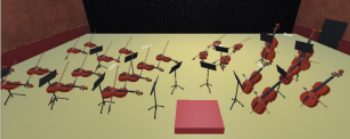
\includegraphics[clip,width=7cm]{gaikan.png}
 \caption{VR弦楽合奏団}\label{fig:gaikan}
\end{figure}
コンテンツの楽曲には,4拍子の曲を用いた.指揮の体験者は両手に持ったコントローラを操作し,音量,曲の再生速度をそれぞれ独立して制御するようにした.再生速度制御に必要なテンポは右手の指揮の動きから推定した.\figref{fig:hyousi}に4拍子の動きとそれを認識する仕 組みを示す.腕がI~IVの順に動いた場合に,4拍子が振れていると認識するようにした.テンポは,60秒を1拍の動作にかかった時間で除算して推定した.

4拍子を表現する腕の動きは,Y座標から検出した1拍の動作に着目し,1拍の間にコントローラが左に移動した場合を1,右に移動した場合を2とし,それを順に記録していく.その並び方が,あらかじめ設定した4拍子のパターンに1つでも該当すれば4拍子ができていると判定した.

 \begin{figure}[b]
 \centering
 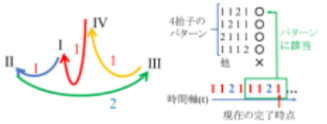
\includegraphics[clip,width=7cm]{hyousi.png}
 \caption{4拍子の動作判定の仕組み}\label{fig:hyousi}
\end{figure}
 
実験では,4拍子の成功や失敗にかかわらず,最後まで演奏を再生するようにした. 

体験者が装着したHMD(Head Mounted Display)を通して観察するコンテンツのシーンを\figref{fig:sikumi}に示す.

 \begin{figure}[b]
 \centering
 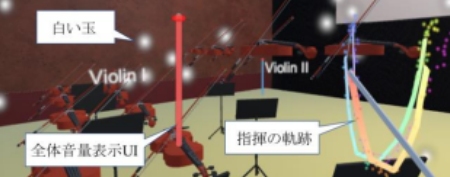
\includegraphics[clip,width=7cm]{sikumi.png}
 \caption{指揮を体験している様子}\label{fig:sikumi}
\end{figure}

また,指揮の成功回数の積み重ねとして示す累積回数に応じて,軌跡の色が「赤→黄→緑→青→紫→ 虹」と変化する.その規則を\figref{fig:sikumi}に示す.

\begin{figure}[t]
 \centering
 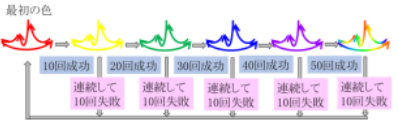
\includegraphics[clip,width=7cm]{sikisikumi.png}
 \caption{指揮軌跡の色の変化の規則}\label{fig:hoge}
\end{figure}



\section{実験}
\subsection{実験方法}
この実験を行う前に予備実験を行った.

この実験では、コンテンツ体験中の被験者の集中力の推移を記録した。集中力の測定は、Neurosky社の脳波計である MindwaveMobile2 を用いて行った。


\section{実験}
\subsection{実験方法}
この実験では、コンテンツ体験中の被験者の集中力の推移を記録した。集中力の測定は、Neurosky社の脳波計である MindwaveMobile2 を用いて行った。


\subsection{実験結果}
4拍子の指揮をする際に指標 UI が効果的に作用し たかどうかについてアンケート調査を行った。図9に結 果を示す。被験者全員から役立ったとの回答が得られ、 指標 UI の表示は有効であることが分かった。 
\begin{figure}[H]
 \centering
 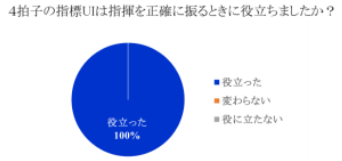
\includegraphics[clip,width=7cm]{UIkouka.png}
 \caption{指揮指標UIの効果}\label{fig:hoge}
\end{figure}

4拍子が正しく 振れているかどうかについて記録したデータを分析し定 量的に調べた。

\begin{figure}[H]
 \centering
 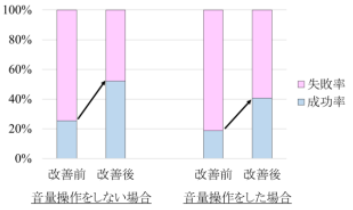
\includegraphics[clip,width=7cm]{sippairitu.png}
 \caption{コンテンツ改善前後の4拍子式の成功比率}\label{fig:hoge}
\end{figure}

\begin{figure}[H]
 \centering
 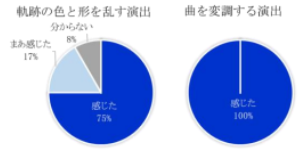
\includegraphics[clip,width=7cm]{miss.png}
 \caption{4拍子失敗時の四角的演出への城の結果}\label{fig:hoge}
\end{figure}

%---------------------------------------------------------------------------
% 本文終わり
%---------------------------------------------------------------------------

 % 参考文献
\bibliographystyle{junsrt}
\bibliography{ref}


\end{document}


%-----------------------------------------------------
% テンプレート
%------------------------------------------------------------------------------

%-----------
%% 箇条書き
%-----------
%\begin{itemize}
% \item
%\end{itemize}

%-------------------
%% 番号付き箇条書き
%-------------------
%\begin{enumerate}
% \item
%\end{enumerate}

%-----------
%% 図の表示
%-----------
%\begin{figure}[H]
% \centering
% \includegraphics[clip,width=7cm]{hoge.eps}
% \caption{図タイトル}\label{fig:hoge}
%\end{figure}

%-----------
%% 図の参照
%-----------
%\figref{fig:hoge}

%-----------
%% 表の作成
%-----------
%\begin{table}[H]
% \centering
% \caption{表タイトル}\label{tab:fuga}
% \begin{tabular}{|c|c|c|}\hline
%  hemo & piyo & fuga \\ \hline
%  hemo & piyo & fuga \\ \hline
% \end{tabular}
%\end{table}

%-----------
%% 表の参照
%-----------
%\tabref{tab:fuga}

%-----------
%% 参考文献
%-----------
%\begin{thebibliography}{9}
% \bibitem{piyo} 参考文献
%\end{thebibliography}

%-----------------
%% 参考文献の参照
%-----------------
%\cite{piyo}
